\documentclass{article}
\usepackage{graphicx}
\usepackage[left=2cm,right=2cm,top=2cm,bottom=2cm]{geometry}
\usepackage{setspace}
\onehalfspacing
\usepackage{float}
\usepackage{fancyhdr}
\usepackage{booktabs}
\usepackage{array}
\usepackage{longtable}
\usepackage{geometry}
\usepackage{amsmath}
\usepackage{amsfonts}
\usepackage{mathrsfs}
\usepackage{hyperref}
\usepackage{listings}
\usepackage{xcolor}

\lstset{
  language=R,
  basicstyle=\ttfamily\small,
  keywordstyle=\color{blue!70},
  commentstyle=\color{gray},
  stringstyle=\color{black},
  rulecolor=\color{gray!40},
  breaklines=true,
  showstringspaces=false,
  numbers=none
}

\fancyhead[LO]{\small{\textit{Risk Theory: Assignment 5}}}

\title{\textbf{Risk Theory 2025/26\\Assignment 5}\\[0.5em]
\textbf{Computing the Loimaranta Efficiency}}
\author{
    Geesink, T. \\
    \texttt{14124165}
    }

\date{May 2026}

\begin{document}
    \pagestyle{fancy}

\includegraphics[scale=0.2]{logo.jpg}
\begingroup
{\let\newpage\relax\maketitle}
\maketitle
\endgroup

\clearpage


\section*{Introduction}
 
If $b(\lambda)$ is the steady-state premium for a driver with claim frequency $\lambda$ in a Markov Bonus Malus (BM) system, the \textit{Loimaranta efficiency} $e(\lambda)$ is the ratio of an infinitesimal percentage change in $b(\lambda)$ to an infinitesimal percentage change in $\lambda$:
 
\begin{equation}
e(\lambda) = \frac{db(\lambda)/b(\lambda)}{d\lambda/\lambda} = \frac{\lambda}{b(\lambda)} \cdot \frac{db(\lambda)}{d\lambda} = \frac{d \log b(\lambda)}{d \log \lambda}
\end{equation}
 
In an ideal BM system, $e(\lambda)$ would be close to 1 for all $\lambda$: a small percentage change in the frequency of claims $\lambda$ would result in the same percentage change in the steady-state premium $b(\lambda)$. But no BM system can achieve this for all $\lambda$.
 
On the right you see a graph of the efficiency $e(\lambda)$ against $\lambda$ of the Dutch 14-step BM system as given in MART Fig. 6.1. We are going to study how $e(\lambda)$ can be computed for a given $\lambda$ from the matrix of transition probabilities $\mathbf{P}$.
 
\subsection*{Three Approaches}
 
We will explore the following three approaches:
 
\begin{itemize}
    \item \textbf{Approximation:} Assuming that after $k$ years the steady state is reached (for a large integer $k$), approximate the steady-state distribution at $\lambda(1 - \varepsilon)$ and at $\lambda(1 + \varepsilon)$ for a small $\varepsilon > 0$, using any row of the $k$-step transition matrix $\mathbf{P}^k$. Then approximate $e(\lambda) = d \log b(\lambda)/d \log \lambda$ by a difference quotient $\Delta \log b(\lambda)/\Delta \log \lambda$.
    
    \item \textbf{Exact:} The steady-state distribution $\ell$, written as a row vector, satisfies the equation $\ell \mathbf{P} = \ell$, so it can be computed exactly as a left-hand eigenvector of $\mathbf{P}$ with eigenvalue 1. Then $b(\lambda(1-\varepsilon))$ and $b(\lambda(1+\varepsilon))$ can be computed exactly, and $e(\lambda)$ can be approximated by a difference quotient as above. Another exact way to get $\ell$ is to use the Rolski--Schmidli--Schmidt--Teugels formula $\ell = \mathbf{1}(\mathbf{I} - \mathbf{P} + \mathbf{1})^{-1}$.
    
    \item \textbf{Simulation:} Use simulated BM positions of the driver after a long period to estimate the steady-state distribution, and from the average premiums paid in the final year, approximate $b(\lambda(1 - \varepsilon))$ and $b(\lambda(1 + \varepsilon))$, then obtain $e(\lambda)$ as a difference quotient.
\end{itemize}
 
\subsection*{Useful Techniques}
 
Some useful techniques you will encounter in this exercise are:
 
\begin{itemize}
    \item linear algebra: matrices, eigenvectors
    \item numerical approximation of derivatives
    \item simulating Markov chains
\end{itemize}
 
\newpage
 
\section{Storing the BM System in R}
 
The script below produces a $4 \times 14$ matrix \texttt{Next} describing which BM class a driver will be in next year, given the driver's current BM class and the number of claims s/he files this year. Also see Table 6.1 in MART. We also define a vector \texttt{BM.frac} that describes what fraction of the basic premium is paid in every BM class.
 
\begin{lstlisting}
## BM class now: 1 2 3 4 5 6 7 8 9 10 11 12 13 14 ## in case of
Next <- rbind(c( 2, 3, 4, 5, 6, 7, 8, 9,10,11, 12,13, 14,14), ## 0 claims
c( 1, 1, 1, 1, 2, 3, 4, 5, 6, 7, 7, 8, 8, 9), ## 1 claim
c( 1, 1, 1, 1, 1, 1, 1, 1, 2, 3, 3, 4, 4, 5), ## 2 claims
c( 1, 1, 1, 1, 1, 1, 1, 1, 1, 1, 1, 1, 1, 1)) ## 3+ claims
BM.frac <- c(120,100,90,80,70,60,55,50,45,40,37.5,35,32.5,30)/100
\end{lstlisting} 
So \texttt{Next[k,a]} = $b$ means that one goes from class $a$ to class $b$ in case of $k-1 = 0,1,2,3+$ claims. For example, the entry \texttt{Next[2,7]} equals 4, so if a driver is in class 7 now, and files 1 claim this year, then she will drop down to class 4 next year. In the vector \texttt{BM.frac} one sees that next year in class 4, this driver will pay 80\% of the base premium instead of the 55\% she is paying this year. \newline
The probability of going from class $i$ to $j$ is $P_{ij} = \sum_k \Pr[\text{$k$ claims}]$, where the sum is taken over all $k$ values that lead to a transition from $i$ to $j$. For example, $P_{7,1} = \Pr[\text{2 claims}] + \Pr[\text{3+ claims}]$, because a transition from class 7 to class 1 is only possible if one files 2 or 3+ claims. The $14 \times 14$ matrix of all transition probabilities $P_{ij}$ is denoted by $\mathbf{P}$. From the vector $p$ containing probabilities of 0, 1, 2, 3+ claims, the transition matrix $\mathbf{P}$ can be constructed (or ``filled'') using the following R function:
 
\begin{lstlisting}
FillP <- function(p) {
  PP <- matrix(0, nrow=14, ncol=14)
  for (b in 1:14) {
    for (k in 1:4) {
      PP[b,Next[k,b]] <- PP[b,Next[k,b]] + p[k] ## k-1 = number of claims
    }
  }
  return(PP)
}
\end{lstlisting}
 
\begin{enumerate}
  \item [$\boldsymbol{Q}_1$]
  \begin{enumerate}
    \item [(a)] Suppose that for a certain driver, the probabilities of $0, 1, 2, 3^+$ claims are $0.65, 0.20, 0.10, 0.05$, respectively. Compute (by hand) the probabilities $P_{7j}$ for $j = 1, \ldots, 14$. \newline
    A:
    \item [(b)] Now compute the probabilities in part (a) using the \lstinline[]|FillP| function, and verify that you get the same results as in part (a). \newline
    A:
\begin{lstlisting}
> P_filled[7,]
[1] 0.15 0.00 0.00 0.20 0.00 0.00 0.00 0.65 0.00 0.00 0.00 0.00 0.00 0.00
\end{lstlisting}
  \end{enumerate}
\end{enumerate}

\clearpage

\section{Approximating the Steady-State Distribution}
 
To approximate the Loimaranta efficiency $e(\lambda) = \frac{d \log b(\lambda)}{d \log \lambda}$, we proceed as follows. Replacing the derivative by a difference quotient, we get:
 
\begin{equation}
e(\lambda) = \frac{d \log b(\lambda)}{d \log \lambda} \approx \frac{\log(b(\lambda(1 + \varepsilon))) - \log(b(\lambda(1 - \varepsilon)))}{\log(\lambda(1 + \varepsilon)) - \log(\lambda(1 - \varepsilon))}, \label{eq:approx}
\end{equation}
for a small $\varepsilon > 0$. In order to apply this approximation for a given $\lambda$ and $\varepsilon$, we need to compute the steady-state premiums $b(\lambda(1 - \varepsilon))$ and $b(\lambda(1 + \varepsilon))$. \newline
Recall that $b(\lambda)$ is the expected premium paid by a driver with claim frequency $\lambda$ in the steady-state distribution. Markov Chain theory tells us that no matter which initial BM class the driver starts in, the distribution of the driver's BM class after many years will converge to the steady-state distribution. In other words, the probability of going from any initial class $i$ to a class $j$ in $k$ steps will converge to the steady-state probability of $j$, as $k \to \infty$. \newline
But the probability of going from $i$ to $j$ in $k$ steps is given by the $(i, j)$ entry of the matrix $\mathbf{P}^k$. For example, if $k = 2$,
 
\begin{equation*}
\Pr[i \to j \text{ in 2 steps}] = \sum_h \Pr[i \to h \to j] \stackrel{\text{Markov}}{=} \sum_h \Pr[i \to h] \Pr[h \to j] = \sum_h P_{ih} P_{hj} = (\mathbf{P}^2)_{ij}.
\end{equation*}
For $k \geq 2$, the same thing can be shown via induction. \newline
We conclude that for large $k$, any row of the matrix $\mathbf{P}^k$ approximates the steady-state distribution (since the initial state does not matter), so the rows of $\mathbf{P}^k$ should be approximately equal, and any one of them can be used as an approximation of the steady-state distribution. We assume that $k = 2^{10} = 1024$ years is large enough to yield a good approximation to the driver's steady-state distribution. \newline \newline
In the R script below, we approximate the Loimaranta efficiency $e(\lambda)$ at $\lambda = 0.05$ via Equation~\ref{eq:approx}. We take $\varepsilon = 0.0001$ and find the steady-state distribution for $\lambda(1 - \varepsilon)$ and $\lambda(1 + \varepsilon)$ as the bottom row of $\mathbf{P}^{1024}$. Note that computing $\mathbf{P}^{1024}$ is easy by taking a square ten times:
 
\[\mathbf{P} \to \mathbf{P}^2 \to (\mathbf{P}^2)^2 = \mathbf{P}^4 \to \mathbf{P}^8 \to \cdots \to \mathbf{P}^{2^{10}} = \mathbf{P}^{1024}.\]
From the steady-state distributions, we compute the corresponding steady-state premiums $b(\lambda(1 - \varepsilon))$ and $b(\lambda(1 + \varepsilon))$, which we then plug into Equation~\ref{eq:approx} to find $e(\lambda)$.
 
\begin{lstlisting}
lam <- 0.05; eps <- 0.0001 ## lambda and epsilon values
lams <- c(lam*(1-eps), lam*(1+eps)) ## where st-state premiums will be computed
b <- c(0,0) ## to store st-state premiums
for (i in 1:2) {
  pp <- dpois(0:2, lams[i]) ## prob of 0, 1, 2 claims
  P <- FillP(c(pp,1-sum(pp))) ## 1-step transition matrix
  for (k in 1:10) {P <- P%*%P} ## P is now P^1024
  stst <- P[nrow(P),] ## bottom row of P is approx st-state dist
  b[i] <- sum(stst*BM.frac) ## st-state premium
}
options(digits=12) ## print many digits, for later comparison
(log(b[2])-log(b[1])) / (log(lams[2])-log(lams[1])) ## e(0.05) = 0.103040331546
\end{lstlisting}
The resulting efficiency value $e(0.05) = 0.103$ is consistent with what we see in the graph on the first page.
\clearpage
\begin{enumerate}
  \item [$\boldsymbol{Q}_2$]
    \begin{enumerate}
      \item [(a)] We want to verify that the 14 rows of $\mathbf{P} = \mathbf{P}^{1024}$ we computed above are indeed (approximately) equal. Rather than printing the matrix $\mathbf{P}$ and checking the equality of rows by visual inspection, we can verify that each column of $\mathbf{P}$ is approximately constant, by applying the \texttt{sd} function to each column, and then displaying the minimum and maximum (i.e. range) of the resulting 14 standard deviations. Fill in the dots to do this, and comment on the output (consult \texttt{?apply} if necessary):
      \begin{lstlisting}
      range(apply(P, ..., ...))
      \end{lstlisting}
      A: \lstinline|range(apply(P, 2, sd))|
\begin{lstlisting}
[1] 1.50351789456e-20 9.73730006967e-17
\end{lstlisting}
      \item [(b)] We also want to verify that $\mathbf{P} = \mathbf{P}^{1024}$ is a proper probability matrix, that is, each row of $\mathbf{P}$ adds up to 1. Fill in the dots to do this, and comment on the output:
      \begin{lstlisting}
      range(apply(P, ..., ...)) - 1
      \end{lstlisting}
      A: \lstinline|range(apply(P, 1, sum)) - 1|
\begin{lstlisting}
[1] 1.06581410364e-14 1.11022302463e-14
\end{lstlisting}
    \end{enumerate}
\end{enumerate}
\clearpage
 
\section{Exact Methods to Find the Steady-State Distribution}
 
\subsection{Using Eigenvectors}
 
In the previous section, we used the rows of $\mathbf{P}^{1024}$ to approximate the steady-state distribution $\ell$. A more exact method is to use the fact that $\ell$ satisfies the equation $\ell \mathbf{P} = \ell$, therefore it is a left-hand eigenvector of $\mathbf{P}$ with eigenvalue 1, with entries that add up to 1. R computes right-hand eigenvectors by default, but that is not a problem because if we transpose both sides of the equality $\ell \mathbf{P} = \ell$, we obtain $\mathbf{P}^\top \ell^\top = \ell^\top$, so $\ell^\top$ is the right-hand eigenvector of the transposed matrix $\mathbf{P}^\top$. So the steady-state distribution can be computed as follows:
 
\begin{lstlisting}
stst <- eigen(t(P))$vectors[,1] ## t(P) is P transposed
stst <- Re(stst/sum(stst)) ## enforce sum=1, take real part only
\end{lstlisting}
Note that \texttt{eigen(t(P))\$vectors} returns the right-hand eigenvectors of $\mathbf{P}^\top$ as columns of a matrix, and the columns are sorted in decreasing order of the corresponding eigenvalues (see \texttt{?eigen}). Since 1 is the largest eigenvalue of $\mathbf{P}^\top$, as explained in MART p. 145, we take the first column of \texttt{eigen(t(P))\$vectors} using the index \texttt{[,1]}. This gives us the eigenvector corresponding to the eigenvalue 1, as we want. Then we scale this vector so that its entries add up to 1, and this is our steady-state vector. \newline \newline
The exact steady-state vectors will lead to exact values for $b(\lambda(1-\varepsilon))$ and $b(\lambda(1+\varepsilon))$, which we can then plug into Equation~\ref{eq:approx} as before to approximate $e(\lambda)$ with a difference quotient. \newline \newline
(In MART Sec. 6.4, a method is described to compute $e(\lambda)$ without relying on difference quotients, but this is not in the scope of this course or this assignment. In any case, this exact method does not lead to much improvement, because the difference quotient (Equation~\ref{eq:approx}) gives the true derivative with an error $O(\varepsilon^2)$, so for example with $\varepsilon = 0.0001$, we get an error of order $10^{-8}$, very much negligible for all applications. For higher precision, $\varepsilon$ can be taken even smaller.)

\begin{enumerate}
  \item [$\boldsymbol{Q}_3$] Compute the value of the Loimaranta efficiency $e(\lambda)$ with $\lambda = 0.05$ and $\varepsilon = 0.0001$ again, by re-running the script before Q2, but this time compute the steady-state vector \texttt{stst} via \texttt{eigen} as described above, instead of approximating it as the bottom row of $\mathbf{P}^{1024}$. The resulting value of $e(0.05)$ should be equal to the one computed above in about 10 digits. \newline
  A:
\begin{lstlisting}
b_eig <- c(0, 0)
for (i in 1:2) {
  pp   <- dpois(0:2, lams[i])
  Ptmp <- FillP(c(pp, 1-sum(pp)))
  stst <- eigen(t(Ptmp))$vectors[, 1]
  stst <- Re(stst / sum(stst))
  b_eig[i] <- sum(stst * BM.frac)
}
e_eig <- (log(b_eig[2])-log(b_eig[1])) / (log(lams[2])-log(lams[1]))
\end{lstlisting}
\begin{lstlisting}
> e_eig
[1] 0.103040331376
> e_pow
[1] 0.103040331585  
\end{lstlisting}
\end{enumerate}
\clearpage
So the rows of $\mathbf{P}^{1024}$ seem to provide an excellent approximation to the steady-state distribution; using exact steady-state distributions barely changes the efficiency value $e(0.05)$.
\subsection{Using the Rolski--Schmidli--Schmidt--Teugels Formula}
 
The second exact way to find the steady-state distribution uses the Rolski--Schmidli--Schmidt--Teugels (RSST) formula. In the slides for Lecture 10 (slide 9), it is shown that the steady-state vector $\ell$ can be computed as $\ell = \mathbf{1}(\mathbf{I} - \mathbf{P} + \mathbf{1})^{-1}$, where $\mathbf{1}$ is a row vector of fourteen 1's, $\mathbf{I}$ is the $14 \times 14$ identity matrix, $\mathbf{1}$ is a $14 \times 14$ matrix of 1's, and $\mathbf{A}^{-1}$ denotes the inverse of matrix $\mathbf{A}$.
 
\begin{enumerate}
  \item [$\boldsymbol{Q}_4$] Compute the value of the efficiency $e(\lambda)$ with $\lambda = 0.05$ and $\varepsilon = 0.0001$ again, by re-running the script before Q2, but this time compute the steady-state vector \texttt{stst} via the RSST formula. The resulting value of $e(0.05)$ should be equal to the one computed in Q3 in about 10 digits. \textit{Hint:} \texttt{diag(14)} produces the $14 \times 14$ identity matrix, \texttt{1} will be interpreted as a matrix of 1's when it is added to another matrix, \texttt{solve(A)} returns the inverse of matrix \texttt{A}. \newline
  A:
\begin{lstlisting}
b_rsst <- c(0, 0)
for (i in 1:2) {
  pp   <- dpois(0:2, lams[i])
  Ptmp <- FillP(c(pp, 1-sum(pp)))
  stst <- rep(1, 14) %*% solve(diag(14) - Ptmp + matrix(1, 14, 14))
  stst <- as.numeric(stst) / sum(stst)
  b_rsst[i] <- sum(stst * BM.frac)
}
e_rsst <- (log(b_rsst[2])-log(b_rsst[1])) / (log(lams[2])-log(lams[1]))
\end{lstlisting}
\begin{lstlisting}
> e_rsst
[1] 0.103040331393
> e_eig
[1] 0.103040331376
\end{lstlisting}
\end{enumerate}
\clearpage

\section{Simulation Method}
 
Finally, we also want to compute the Loimaranta efficiency by simulation. For a given driver with claim frequency $\lambda$, we simulate many BM histories (say 10,000) spanning a period sufficiently long (say 100 years) to eliminate the effect of the starting class. The final BM class the driver ends up in after 100 years should be a random drawing from the steady-state distribution, so the distribution of the 10,000 final BM classes is an approximation for the steady-state distribution, and the average premium paid in those 10,000 final BM classes is an estimate for $b(\lambda)$. \newline
In the script below, we apply this idea to estimate the value of $b(\lambda)$ for $\lambda = 0.05$. We produce a stream of Poisson($\lambda$) claim numbers for 100 years, and move the driver among the BM classes according to these claim numbers and the \texttt{Next} matrix, starting from BM class 14. Then we produce a table of the final BM classes the driver ends up in, which is an estimate of the steady-state distribution, as well as the mean and standard deviation of the premium paid in the final year. The mean is an estimate for $b(\lambda)$.
 
\begin{lstlisting}
options(digits=6); set.seed(666)
TMax <- 100; NSim <- 10000; FinalBM <- rep(0,NSim); lam <- 0.05
for (n in 1:NSim) {
  cn <- rpois(TMax,lam) ## 100 claim numbers for 100 years
  cn <- pmin(cn,3) + 1 ## convert claim nbrs into 1,2,3,4 for 0,1,2,3+ claims
  BM <- 14 ## start in BM class 14
  for (i in 1:TMax) {BM <- Next[cn[i],BM]} ## move among classes for 100 years
  FinalBM[n] <- BM ## the final BM class at the end of 100 years
}
100*table(FinalBM)/NSim ## percentage of sim's that ended up in class 1,...,14
## 1 2 3 4 5 6 7 8 9 10 11 12 13 14
## 0.02 0.03 0.10 0.09 0.18 0.37 0.74 1.25 4.54 4.53 4.35 4.00 3.53 76.27
mean(BM.frac[FinalBM]) ## 0.325, the estimate for b(0.05)
sd(BM.frac[FinalBM]) ## 0.061
\end{lstlisting}
The Loimaranta efficiency $e(\lambda)$ can now be estimated as a difference quotient as in Equation~\ref{eq:approx}, where both $b(\lambda(1 - \varepsilon))$ and $b(\lambda(1 + \varepsilon))$ are estimated via 10,000 simulations as above. \newline
How precise is the estimate for $b(\lambda)$ when we use 10,000 simulations? Let $X_i$ denote the premium paid in the final BM class in the $i$-th simulation run. We estimate $b(\lambda) = \mathbb{E}[X_i]$ as $\bar{X}$, the average of the $X_i$ values. By the Central Limit Theorem, $\bar{X}$ is normal with mean $\mu_{X_i} = b(\lambda)$ and standard deviation $\sigma_{X_i}/\sqrt{10,000} \approx 0.061/100$. This implies that there is about 99\% chance that the $b(\lambda)$ estimate $\bar{X}$ will lie inside the interval $(0.995 b(\lambda), 1.005 b(\lambda))$.
\clearpage
\begin{enumerate}
  \item [$\boldsymbol{Q}_5$] Use any technique described in Section 2 or 3 above ($\mathbf{P}^{1024}$, \texttt{eigen()}, RSST) to compute the steady-state premium $b(0.05)$ more precisely, and verify that the simulation estimate 0.325 indeed lies in the interval $(0.995 b(0.05), 1.005 b(0.05))$. \newline
  A:
\begin{lstlisting}
pp      <- dpois(0:2, 0.05)
Ptmp    <- FillP(c(pp, 1-sum(pp)))
stst_ex <- rep(1,14) %*% solve(diag(14) - Ptmp + matrix(1,14,14))
stst_ex <- as.numeric(stst_ex) / sum(stst_ex)
b_exact <- sum(stst_ex * BM.frac)
\end{lstlisting}
\begin{lstlisting}
> b_sim
[1] 0.325105
> b_exact
[1] 0.326079
> b_sim >= 0.995*b_exact & b_sim <= 1.005*b_exact
[1] TRUE
\end{lstlisting}
\end{enumerate}
\clearpage
So it might seem like the simulation estimate of $b(\lambda)$ is precise enough, but to estimate the efficiency $e(\lambda) = \frac{d \log b(\lambda)}{d \log \lambda}$, it turns out to be much too crude. Indeed, assume that $b(\lambda(1+\varepsilon))$ is estimated as, for example, $0.998 b(\lambda(1 +\varepsilon))$, and $b(\lambda(1-\varepsilon))$ is estimated as $1.002 b(\lambda(1-\varepsilon))$. Then we get the following estimate for $e(\lambda)$:
 
\begin{equation}
\frac{\log (0.998 b(\lambda(1 + \varepsilon))) - \log (1.002 b(\lambda(1 - \varepsilon)))}{\log(\lambda(1 + \varepsilon)) - \log(\lambda(1 - \varepsilon))} \approx e(\lambda) - \frac{0.004}{2\varepsilon} = e(\lambda) - \frac{1}{500\varepsilon}. \label{eq:error}
\end{equation}
Taking $\varepsilon = 10^{-4}$ as before gives an estimation error of $\frac{1}{500\varepsilon} = 20$, clearly unacceptable.
 
\begin{enumerate}
  \item [$\boldsymbol{Q}_6$]
  \begin{enumerate}
    \item [(a)] Use $\log xy = \log x + \log y$ and $\log(1 + x) \approx x$ for small $|x|$, as well as Equation~\ref{eq:approx}, to prove the approximation in Equation~\ref{eq:error}. \newline
    A:
    \item [(b)] Estimate the efficiency $e(\lambda)$ with $\lambda = 0.05$ and $\varepsilon = 0.0001$ using simulations. Adapt the script given above to estimate both $b(\lambda(1-\varepsilon))$ and $b(\lambda(1+\varepsilon))$ via $NSim = 10,000$ simulations, and then apply Equation~\ref{eq:approx} to find $e(\lambda)$. Repeat this procedure five times to get five $e(\lambda)$ estimates. How do they compare with the $e(\lambda)$ value we computed in Q3/Q4? \newline
    A:
\begin{lstlisting}
sim_b <- function(lam_val, NSim=10000, TMax=100) {
  fbm <- integer(NSim)
  for (n in 1:NSim) {
    cn  <- pmin(rpois(TMax, lam_val), 3) + 1L
    BM  <- 14L
    for (i in 1:TMax) BM <- Next[cn[i], BM]
    fbm[n] <- BM
  }
  mean(BM.frac[fbm])
}

sim_e <- function(lam, eps_val, NSim=10000, TMax=100) {
  lv <- c(lam*(1-eps_val), lam*(1+eps_val))
  bv <- c(sim_b(lv[1], NSim, TMax),
          sim_b(lv[2], NSim, TMax))
  (log(bv[2]) - log(bv[1])) / (log(lv[2]) - log(lv[1]))
}
\end{lstlisting}
\begin{lstlisting}
> e6b
[1] 14.85771 19.04268  3.91471 15.81934 14.98137
> e_rsst
[1] 0.10304
\end{lstlisting}
    
    \item [(c)] Repeat part (b), but now with $\varepsilon = 0.1$. How do the $e(\lambda)$ estimates compare with the value in Q3/Q4? \newline
    A:
\begin{lstlisting}
> e6c
[1] 0.1066559 0.0994235 0.1161507 0.0921594 0.0943348
> e_rsst
[1] 0.10304
\end{lstlisting}
  \end{enumerate}
\end{enumerate}

\clearpage
 
So to get sufficiently precise results, the error in the estimates of $b(\lambda(1 - \varepsilon))$ and $b(\lambda(1 + \varepsilon))$ must be strongly reduced, meaning that many more simulations have to be done. That is unfortunate, because the value of $e(\lambda)$ is generally needed for many $\lambda$ values, for instance to produce a graph of $e(\lambda)$, as in the first page of this assignment, or to compute $\max_\lambda e(\lambda)$, or $\int e(\lambda) \, dU(\lambda)$ for some structure distribution $U(\cdot)$.
 
\section{Some Commercially Attractive Variations}
 
Suppose the marketing department of a certain insurer has two ideas to attract extra customers. These ideas are as follows:
 
\begin{enumerate}
    \item \textbf{Waiving a claim in leap years:} In each leap year 2028, 2032, 2036, \ldots, the first claim is simply paid for by the insurer, without consequences for the position in the BM ladder.
    
    \item \textbf{Bonus guarantee:} Extra classes 15, \ldots, 20 are added to the BM-ladder, each with the same premium as class 14. A driver in class 14 keeps climbing up the BM-ladder one class at a time for each claim-free year, and drops down the same number of classes as in class 14 in case of $\geq 1$ claims. The rationale behind this is that it is considered unfair to lose one's no-claim discount by having a claim after twenty or more claim-free years.
\end{enumerate}
 
The management wants an estimate from the actuarial department of the financial consequences of these ideas. Specifically, they want to know how much less a typical driver having $\lambda = 0.05$ will pay on average, assuming the steady-state distribution over the BM classes.
 
\subsection{Waiving the First Claim in Leap Years}
 
To analyze this modification of the BM-scheme, we have to resort to simulations since the Markov analysis does not apply anymore, with the transition matrix changing every 4 years. For simplicity, we will consider every year divisible by 4 to be a leap year (even though in reality, years divisible by 100 are not leap years, unless they are also divisible by 400). We will also pretend that we are now at the beginning of 2025, so the leap year bonus will apply to years 4, 8, 12, \ldots
\clearpage
\begin{enumerate}
  \item [$\boldsymbol{Q}_7$] Adapt the script provided in Section 4 to compute an estimate for the steady-state premium $b(0.05)$ in the modified BM-scheme. How does the new steady-state premium compare with the original one? (\textit{Hint:} Use again 10,000 simulated claim histories of 100 years, with the same random seed \texttt{set.seed(666)} as in the earlier script. Using the same seed will produce the exact same claim histories, so we can compare the results from the two BM-schemes for the same claim histories. In years 4, 8, 12, \ldots, 100, reduce the number of claims (if positive) by one, by using partial replacement: \texttt{cn[(1:25)*4] <- \ldots cn[(1:25)*4] \ldots}) \newline
  A: 
\begin{lstlisting}
NSim <- 10000;  TMax <- 100;  lam <- 0.05
FinalBM_leap <- integer(NSim)
for (n in 1:NSim) {
  cn <- pmin(rpois(TMax, lam), 3) + 1L
  cn[(1:25)*4] <- pmax(1L, cn[(1:25)*4] - 1L)
  BM <- 14L
  for (i in 1:TMax) BM <- Next[cn[i], BM]
  FinalBM_leap[n] <- BM
}
b_leap <- mean(BM.frac[FinalBM_leap])
\end{lstlisting}
\begin{lstlisting}
> b_sim
[1] 0.325105
> b_leap
[1] 0.314527
> round(100*(b_sim - b_leap)/b_sim, 3)
[1] 3.254
\end{lstlisting}
\end{enumerate}
\clearpage

\subsection{Bonus Guarantee}
 
In this modification, additional BM classes 15, \ldots, 20 are added to the original 14-class system, and a driver in class 14 keeps climbing up one class at a time for each claim-free year. When in class 20 and claim-free, one remains in class 20. In each of these new classes, the driver pays the same premium as in class 14, i.e. 30\% of the base premium. By making one claim, one falls back from class $k \geq 14$ to $k - 5$. By two claims, one goes to $k - 9$, by three or more, to $k - 13$. The rules for classes $k \leq 13$ remain the same as before.
 
Since the Markov chain structure is still maintained (albeit with 20 classes instead of 14), we can get exact results without resorting to simulations.
 
\begin{enumerate}
  \item [$\boldsymbol{Q}_8$]
  \begin{enumerate}
    \item [(a)] Define a new matrix \texttt{Next20} and a new vector \texttt{BM.frac20} for this extended BM system, analogous to \texttt{Next} and \texttt{BM.frac} defined in Section 1 for the 14-class system. \newline
    A:
\begin{lstlisting}
Next20 <- rbind(
  c(2,3,4,5,6,7,8,9,10,11,12,13,14,15,16,17,18,19,20,20),
  c(1,1,1,1,2,3,4,5, 6, 7, 7, 8, 9,10,11,12,13,14,15,15),
  c(1,1,1,1,1,1,1,1, 2, 3, 3, 4, 5, 6, 7, 8, 9,10,11,11),
  c(1,1,1,1,1,1,1,1, 1, 1, 1, 1, 2, 2, 3, 4, 5, 6, 7, 7)
)

BM.frac20 <- c(120,100,90,80,70,60,55,50,45,40,37.5,35,32.5, rep(30,7)) / 100
\end{lstlisting}
    \item [(b)] Define a new function \texttt{FillP20} for this extended BM system, analogous to \texttt{FillP} defined in Section 1.\textit{Hint:} \texttt{FillP20} should produce a $20 \times 20$ matrix instead of $14 \times 14$, and it should use the \texttt{Next20} matrix instead of \texttt{Next}. \newline
    A:
\begin{lstlisting}
FillP20 <- function(p) {
  PP <- matrix(0, nrow=20, ncol=20)
  for (b in 1:20)
    for (k in 1:4)
      PP[b, Next20[k,b]] <- PP[b, Next20[k,b]] + p[k]
  return(PP)
}
\end{lstlisting} \clearpage
    \item[(c)] Use any technique described in Section 2 or 3 above ($\mathbf{P}^{1024}$, \texttt{eigen()}, RSST) to find the steady-state premium $b(0.05)$ in this extended BM system. How does the new steady-state premium compare with the original one? \newline
    A: 
\begin{lstlisting}
pp     <- dpois(0:2, 0.05)
pv     <- c(pp, 1-sum(pp))
P20    <- FillP20(pv)
stst20 <- rep(1,20) %*% solve(diag(20) - P20 + matrix(1,20,20))
stst20 <- as.numeric(stst20) / sum(stst20)
b_ext  <- sum(stst20 * BM.frac20)
\end{lstlisting}
\begin{lstlisting}
[1] 0.326079
> b_ext
[1] 0.301791
> round(b_ext/b_exact, 5)
[1] 0.92552
> round(100*(1 - b_ext/b_exact), 2)
[1] 7.45
\end{lstlisting}
  \end{enumerate}
\end{enumerate}
\clearpage
 
We see from the previous question that in the extended system, the steady-state premium $b(0.05)$ drops to about 93\% of its original value. We would also like to see how much the steady-state premium $b(\lambda)$ drops for other $\lambda$ values in the interval $(0, 0.5]$.
 
\begin{enumerate}
  \item [$\boldsymbol{Q}_9$]
  \begin{enumerate}
    \item [(a)] Consider the 100 values $\lambda = 1/200, 2/200, \ldots, 100/200$ in the interval $(0, 0.5]$. Write a loop that computes the steady-state premium $b(\lambda)$ in the original (14-class) BM system as well as the steady-state premium $b^*(\lambda)$ in the extended (20-class) BM system for each of these $\lambda$ values, and store the proportions $b^*(\lambda)/b(\lambda)$ in a vector of length 100 called \texttt{prop}. (You can use any technique described in Section 2 or 3 to compute steady-state premiums.)
 
    \begin{lstlisting}
    lambdas <- 1:100/200
    prop <- rep(0,100)
    for (i in 1:100) {
      ...
    }
    \end{lstlisting}
    A:
\begin{lstlisting}
lambdas <- 1:100/200
prop    <- numeric(100)

for (i in 1:100) {
  la <- lambdas[i]
  pv <- c(dpois(0:2, la), 1 - sum(dpois(0:2, la)))
  
  Pt  <- FillP(pv)
  st  <- rep(1,14) %*% solve(diag(14) - Pt  + matrix(1,14,14))
  st  <- as.numeric(st)  / sum(st)
  
  P20t <- FillP20(pv)
  st20 <- rep(1,20) %*% solve(diag(20) - P20t + matrix(1,20,20))
  st20 <- as.numeric(st20) / sum(st20)
  
  prop[i] <- sum(st20 * BM.frac20) / sum(st * BM.frac)
}
\end{lstlisting} \clearpage
    \item [(b)] Produce a plot of the proportions you computed in part (a) against $\lambda$. Which drivers would benefit most from the adoption of the extended BM system? \newline
    A:
    \begin{center}
      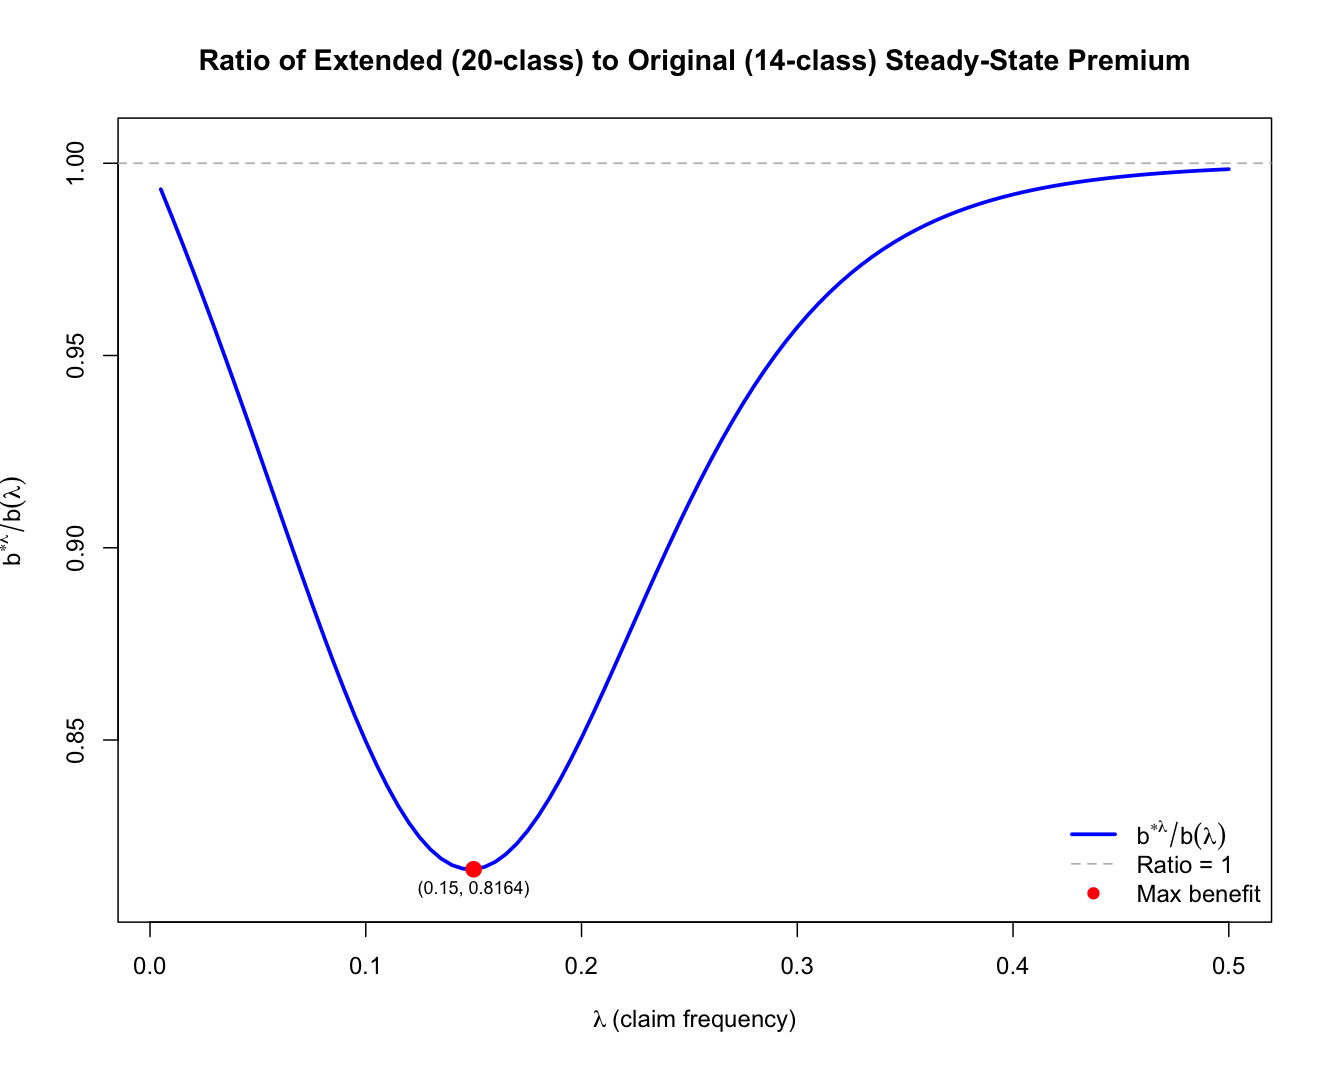
\includegraphics[width=0.7\textwidth]{Assignment 5 Q9b.png}
    \end{center}
    The ratio is lowest ($\approx$ 0.816) around $\lambda$ = 0.15. Drivers with an intermediate claim frequency (about 1 claim every 6-7 years) benefit most: they file occasional claims so cannot easily stay at class 14 in the original system, but with the bonus guarantee they can reach classes 15-20 and recover there after a claim. Very low-$\lambda$ drivers already sit permanently at class 14 (little to gain). Very high-$\lambda$ drivers claim so often that the extra classes offer little shelter.

  \end{enumerate}
\end{enumerate}
\end{document}